\documentclass[a4paper]{article}
\input{~/preamble.tex}

\title{Βάσεις Δεδομένων \\ Σειρά Ασκήσεων}
\author{\textbf{Ομάδα Μ} \\~\\ Νικήτας Τσίννας, el18187 \\ Αναστάσιος Παπαζαφειρόπουλος, el18079 \\ Νικόλαος Παγώνας, el18175}
\date{}

\setlength{\parskip}{0em}

\begin{document}

\maketitle

\subsection*{Exercise 1}

\subsubsection*{A.}

\begin{figure}[H]
	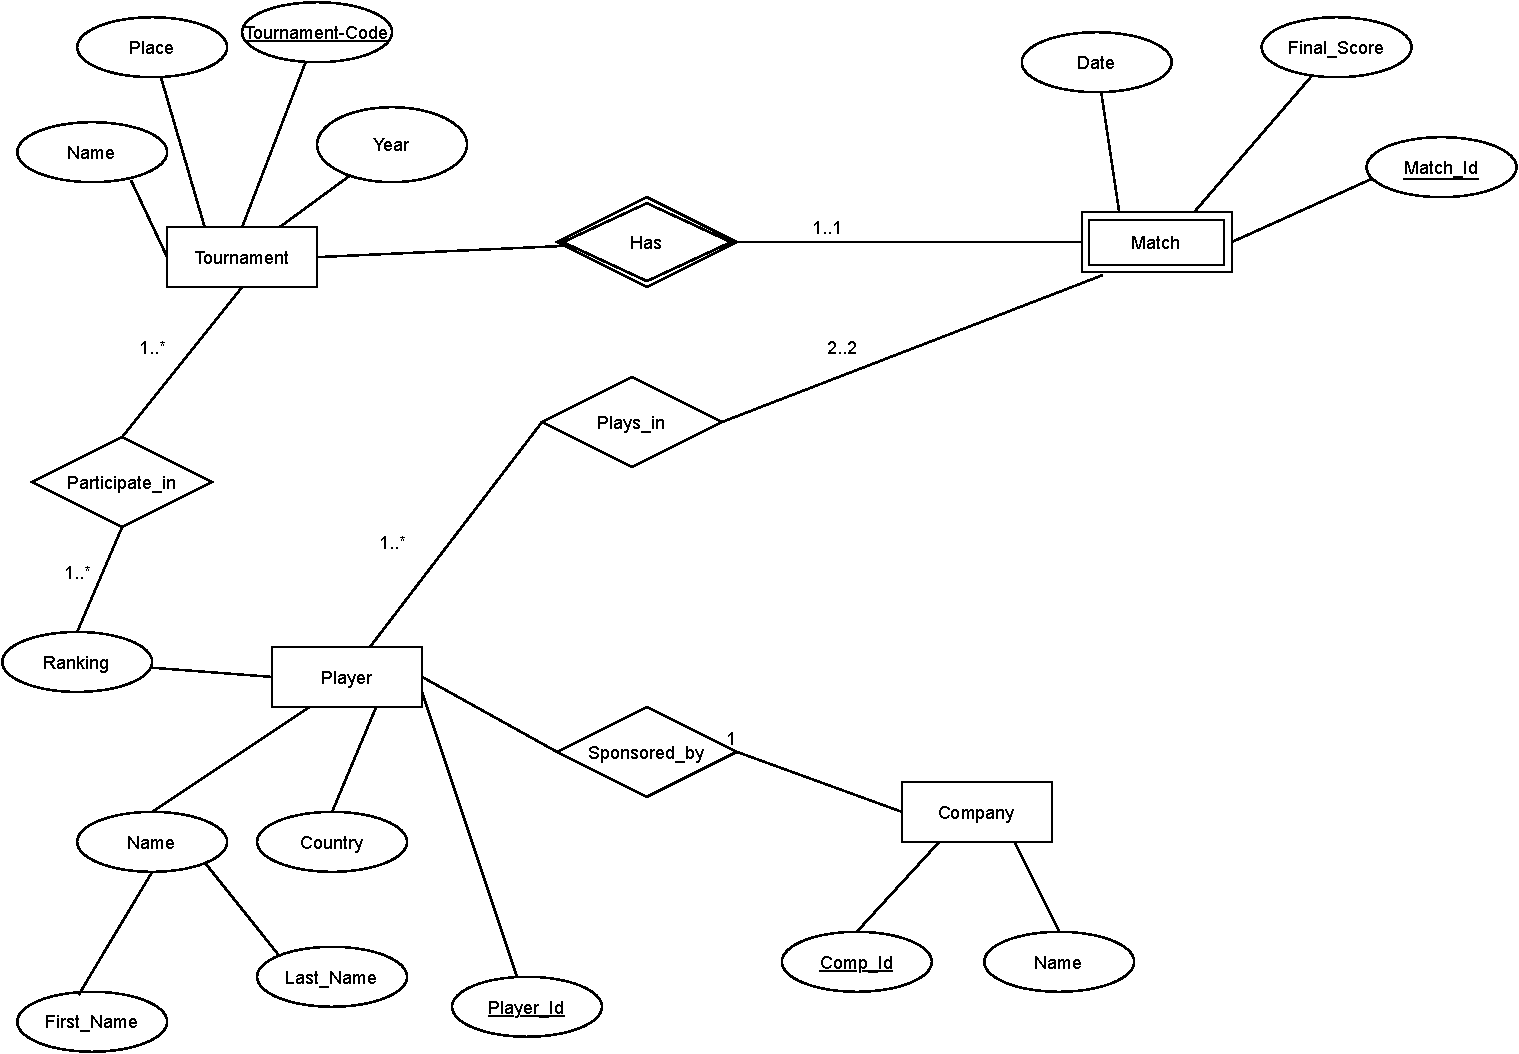
\includegraphics[width=\textwidth]{ex1_ER_final.pdf}
\end{figure}

Στο παραπάνω διάγραμμα ER υπάρχουν:

\begin{itemize}
	\item Το σύνολο οντοτήτων Tournament με Attributes: Name, Place, Year, Tournament-Code και primary key: Tournament-Code που θα κωδικοποιεί μοναδικά το τουρνουά. Αυτό είναι απαραίτητο γιατί καμία άλλη πληροφορία δε μπορεί να καθορίσει μοναδικά ένα τουρνουά.
	\item Το σύνολο οντοτήτων Player με Attributes: Name(First\_Name, Last\_Name), Country, Ranking και Player\_Id, το οποίο θα μπορούσε να είναι για παράδειγμα ο αριθμός ταυτότητας εξαρτάται από τους διοργανωτές. Αυτό είναι και το primary key μιας και εδώ καμία από τις υπόλοιπες πληροφορίες δε μπορεί να καθορίσει μοναδικά έναν παίκτη.
	\item Το σύνολο οντοτήτων Company με Attributes: Name, Comp\_Id και primary key: Comp\_Id.
	\item Η N:M σχέση Participate\_in που συνδέει το Tournament με το Player, καθώς πολλοί παίκτες μπορούν να συμμετέχουν σε ένα τουρνουά, αλλά και ένας παίκτης να συμμετέχει σε πολλά τουρνουά. Επίσης, η σχέση αυτή είναι total participation ως προς τον Player και ως προς το τουρνουά, καθώς δε γίνεται να υπάρξει τουρνουά χωρίς παίκτες από τη μία και από την άλλη θεωρήσαμε ότι δε γίνεται ένας παίκτης να μην έχει συμμετάσχει ποτέ σε τουρνουά, γιατί τότε δε θα θεωρούνταν παίκτης.
	\item Η 1:Ν σχέση Sponsored\_by που συνδέει το Player με το Company.
	\item To αδύναμο σύνολο οντοτήτων Match με Attributes: Date, Final\_Score και Match\_Id. Είναι αδύναμο, καθώς υλοποιήθηκε με τη λογική ότι κάθε match αναφέρεται σε ένα τουρνουά στο οποίοπραγματοποιήθηκε, άρα και δε μπορεί να καθοριστεί χωρίς το primary key του Tournament (Tournament\_Code). 
	\item H 2:Ν σχέση Plays που συνδέει το Player με το Match, καθώς δύο παίκτες αγωνίζονται σε κάθε παιχνίδι. Επίσης, εδώ θεωρήσαμε ότι δε γίνεται να υπάρξει παίκτης που να μην έχει δώσει ποτέ παιχνίδι. 
\end{itemize}

\subsubsection*{B.}

	Από το παραπάνω  ER διάγραμμα προκύπτουν:
	
	\begin{itemize}
		\item Player(\uline{Player\_Id}, First\_Name, Last\_Name, Country, Ranking, \dashuline{Comp\_Id}) \\
		
		με foreign key: Comp\_Id, καθώς η σχέση Sponsored\_By είναι 1:N
		\item Company(\uline{Comp\_Id}, Name) \\
		
		\item Tournament(Tournament\_Code, Name, Place, Year)  \\
		\item Match(\uline{Match\_Id}, \dashuline{Tournament\_Code}, Date, Final\_Score) \\ 
		
		με foreign key: Tournament Code ως πρωτεύον κλειδί της ισχυρής οντότητας.
		\item Participates\_in(\uline{\dashuline{Player\_Id}}, \uline{\dashuline{Tournament\_Code}}), καθώς η σχέση αυτή στο ER είναι  Ν:Μ, με primary \\
		
		και foreign keys, τα  primary keys των οντοτήτων που συνδέονται.
		\item Plays\_in(\uline{\dashuline{Player\_Id}}, \uline{\dashuline{Match\_Id}}), καθώς η σχέση αυτή στο ER είναι 2:Ν, με primary και foreign keys, \\
		
		τα  primary keys των οντοτήτων που συνδέονται.
	\end{itemize}

\subsection*{Exercise 2}

$Q_1:$
\[
	\scalebox{1.5}{$\Pi$}_{\text{pid}}(\scalebox{1.5}{$\sigma$}_{\text{companyname=''Google''}}(\text{Person} \bowtie \text{Company})) \ \scalebox{1.5}{$\cap$} 
\]

\[
	\scalebox{1.5}{$\Pi$}_{\text{pid}}(\scalebox{1.5}{$\sigma$}_{\text{sharenum} >  \text{500}}(\scalebox{1.5}{$\sigma$}_{\text{companyname=''Facebook''}}(\text{Shares} \ \bowtie \ \text{Company})))
\]

$Q_2:$
\[
	\scalebox{1.5}{$\Pi$}_{\text{Person.pid}}(\scalebox{1.5}{$\sigma$}_{\text{Person.cid = Shares.cid} \land \text{Person.managerid = Shares.pid} \land \text{Sharesnum} > \text{0}}(\text{Person} \times \text{Shares}))
\]

$Q_3:$
\[
	\scalebox{1.5}{$\Pi$}_{\text{pid}}(_{_{\text{\scriptsize pid}}}\scalebox{2}{$g$}_{\text{(count(cid)}>\text{2})}(\scalebox{1.5}{$\sigma$}_{\text{sharesnum} > \text{0}}(\text{Shares})))
\]

$Q_4:$
\[
	\scalebox{1.5}{$\Pi$}_{\text{pid,cid}}(\scalebox{1.5}{$\sigma$}_{\text{sharesnum} > \text{0}}(Shares)) \ \scalebox{1.5}{$/ \ \Pi$}_{\text{cid}}(Company)
\]



\subsection*{Exercise 3} ~\\

\begin{minipage}{\linewidth}
Q1: \\

Βρες το id και το όνομα των καταστημάτων που στεγάζουν λιγότερο από 100 υπαλλήλους ή βρίσκονται στην Αθήνα. \\

\textbf{select} s.sname \\

\textbf{from} Store \textbf{as} s \\

\textbf{where} city='Athens' \textbf{or} employee\_number $<=$ 100 \\
\end{minipage}

\begin{minipage}{\linewidth}
Q2: \\

Βρες το όνομα των καταστημάτων που προμηθεύονται μολύβια \\

\textbf{select} st.sname \\

\textbf{from} store \textbf{as} st \\
\textbf{inner} \textbf{join} (supply \textbf{as} su  

    ~~~~\textbf{inner} \textbf{join} Goods \textbf{as} g 
     
    ~~~~\textbf{on} g.gid=su.gid) \\
\textbf{on} st.storeid = su.storeid \\

\textbf{where} gname='μολύβι' \\

\end{minipage}

\begin{minipage}{\linewidth}
Q3: \\

Βρες το όνομα και την πόλη των καταστημάτων που προμηθεύονται τα προϊόντα που προμηθεύεται το κατάστημα με id=0808. \\

\textbf{select} st.sname, st.city \\

\textbf{from} supply \textbf{as} su \\

\textbf{where} \textbf{not} \textbf{exists}( 

	~~~~(\textbf{Select} su1.gid 
	
	~~~~\textbf{from} supply \textbf{as} su1 
	
	~~~~\textbf{where} su1.storeid = 0808) \\
	

	~~~~\textbf{except} \\
	

	~~~~(\textbf{select} su2.gid 
	
	~~~~\textbf{from} supply \textbf{as} su2 
	
	~~~~\textbf{where} su2.storeid = st.storeid 
	
) \\

\end{minipage}

\begin{minipage}{\linewidth}
Q4: \\

\textbf{with} aux \textbf{as} (

    ~~~~\textbf{select} \textbf{count}(su.gid) \textbf{as} total\_goods, su.storeid
    
    ~~~~\textbf{from} Supply \textbf{as} su
    
    ~~~~\textbf{group} \textbf{by} su.storeid
    
    ~~~~\textbf{order} \textbf{by} total\_goods \textbf{desc}
    
    ~~~~\textbf{limit} 5) \\
    

\textbf{select} \textbf{distinct} st.sname\\

\textbf{from} Store \textbf{as} st
\textbf{natural} \textbf{join} aux\\

\end{minipage}

\begin{minipage}{\linewidth}
Q5: \\

\textbf{select} st.city\\

\textbf{from} store \textbf{as} st\\
\textbf{inner} \textbf{join} (supply \textbf{as} su

    ~~~~\textbf{inner} \textbf{join} goods \textbf{as} g
    
    ~~~~\textbf{on} g.gid = su.gid)
    
\textbf{on} st.storeid = su.storeid\\

\textbf{having} \textbf{max}(price)$>$\textbf{200}\\

\end{minipage}

\begin{minipage}{\linewidth}
Q6: \\

\textbf{select} \textbf{distinct} su.gid \\

\textbf{from} (Supply as su \textbf{inner} \textbf{join} Store as st \textbf{on} su.storeid = st.storeid) \\
\textbf{inner} \textbf{join} Goods as g \\
\textbf{on} su.gid = g.gid \\

\textbf{where} st.city = 'Athens' \\
\textbf{group} \textbf{by} su.gid \\
\textbf{having} \textbf{count} (su.storeid) = (\textbf{select} \textbf{count}(storeid) 

~~~~\textbf{from} Store \textbf{as} st

~~~~\textbf{where} st.city = 'Athens')\\

\end{minipage}

\begin{minipage}{\linewidth}
Q7: \\

(\textbf{select} gid\\

\textbf{from} store \textbf{as} st \\
\textbf{natural} \textbf{join} supply \textbf{as} su\\

\textbf{where} st.city = 'Athens')\\

\textbf{except}\\

(\textbf{select} gid\\

\textbf{from} Store \textbf{as} st\\
\textbf{natural} \textbf{join} Supply \textbf{as} su\\

\textbf{Where} st.city = 'Patras')\\

\end{minipage}

\subsection*{Exercise 4}

\subsubsection*{A.}

Find all attributes that have not appeared on the RHS of any FD: $ S_1 = \{B,C\}$ 

Find all attributes that have not appeared on the LHS of any FD: $ S_2 = \{A\}$ \\

Compute the closure set of $S_1$: $S_1^+ = \{A, B, C, D, E\}$. \\

$ S_1^+ = R $, so $ \{B, C\} $ is the only candidate key.  


\subsubsection*{B.}

Computing a canonical cover for F: \\

Initially, $ F_c = F $. \\

	Iteration \#1: \\
	
	~~~~ Can't use union rule. \\
	
	~~~~ Checking $B\rightarrow EA:$  \\
	
	~~~~ ~~~~ Removing B: 
	
	~~~~ ~~~~ ~~~~ $ \varnothing^+=\varnothing $, doesn't contain B, so B is needed. \\
	
	~~~~ ~~~~ 	Removing E: 
	
	~~~~ ~~~~ ~~~~ $ F_c'=\{B\rightarrow A, EBC \rightarrow D, BED \rightarrow A\}$ 
	
	~~~~ ~~~~ ~~~~ $ (B)^+=(AB) $, doesn't contain E, so E is needed. \\
				
	~~~~ ~~~~ 	Removing A: 
	
	~~~~ ~~~~ ~~~~ $ F_c'=\{B\rightarrow E, EBC \rightarrow D, BED \rightarrow A\}$ 
	
	~~~~ ~~~~ ~~~~ $ (B)^+=(BE) $, doesn't contain A, so A is needed. \\
				
	~~~~ Checking $EBC\rightarrow D:$ \\
		
	~~~~ ~~~~ Removing E: 
	
	~~~~ ~~~~ ~~~~ $ (BC)^+=(ABCDE) $, contains E, so E is extraneous in $EBC\rightarrow D$. \\
	
	~~~~ Now $F_c = \{B \rightarrow EA, BC \rightarrow D, BED \rightarrow A\}$ \\
	
	Iteration \#2: \\
	
	~~~~ Can't use union rule. \\
	
	~~~~ Checking $B\rightarrow EA:$ \\
		
	~~~~ ~~~~ Removing B: 
	
	~~~~ ~~~~ ~~~~ $ \varnothing^+=\varnothing $, doesn't contain B, so B is needed. \\
		
	~~~~ ~~~~ Removing E: 
	
	~~~~ ~~~~ ~~~~ $ F_c'=\{B\rightarrow A, BC \rightarrow D, BED \rightarrow A\}$ 
	
	~~~~ ~~~~ ~~~~ $ (B)^+=(AB) $, doesn't contain E, so E is needed. \\
		
	~~~~ ~~~~ Removing A: 
	
	~~~~ ~~~~ ~~~~ $ F_c'=\{B\rightarrow E, BC \rightarrow D, BED \rightarrow A\}$ 
	
	~~~~ ~~~~ ~~~~ $ (B)^+=(BE) $, doesn't contain A, so A is needed. \\
		
	~~~~ Checking $BC\rightarrow D:$ \\
		
	~~~~ ~~~~ Removing B: 
	
	~~~~ ~~~~ ~~~~ $ (C)^+=(C) $, doesn't contain B, so B is needed. \\
		
	~~~~ ~~~~ Removing C: 
	
	~~~~ ~~~~ ~~~~ $ (B)^+=(ABE) $, doesn't contain C, so C is needed. \\
		
	~~~~ ~~~~ Removing D: 
	
	~~~~ ~~~~ ~~~~ $ F_c'=\{B\rightarrow EA, BED \rightarrow A\}$ 
	
	~~~~ ~~~~ ~~~~ $ (BC)^+=(ABCE) $, doesn't contain D, so D is needed. \\
		
	~~~~ Checking $BED\rightarrow A:$ \\
		
	~~~~ ~~~~ Removing B: 
	
	~~~~ ~~~~ ~~~~ $ (ED)^+=(ED) $, doesn't contain B, so B is needed. \\
		
	~~~~ ~~~~ Removing E: 
	
	~~~~ ~~~~ ~~~~ $ (BD)^+=(ABDE) $, contains E, so E is extraneous in $ BED \rightarrow A $. \\
	
	~~~~ Now $F_c = \{B \rightarrow EA, BC \rightarrow D, BD \rightarrow A\}$ \\
	
	Iteration \#3: \\
	
	~~~~ Can't use union rule. \\
	
	~~~~ Checking $B\rightarrow EA:$ \\
		
	~~~~ ~~~~ Removing B: 
	
	~~~~ ~~~~ ~~~~ $ \varnothing^+=\varnothing $, doesn't contain B, so B is needed. \\
		
	~~~~ ~~~~ Removing E: 
	
	~~~~ ~~~~ ~~~~ $ F_c'=\{B\rightarrow A, BC \rightarrow D, BD \rightarrow A\}$ 
	
	~~~~ ~~~~ ~~~~ $ (B)^+=(AB) $, doesn't contain E, so E is needed. \\
		
	~~~~ ~~~~ Removing A: 
	
	~~~~ ~~~~ ~~~~ $ F_c'=\{B\rightarrow E, BC \rightarrow D, BD \rightarrow A\}$ 
	
	~~~~ ~~~~ ~~~~ $ (B)^+=(BE) $, doesn't contain A, so A is needed. \\
		
	~~~~ Checking $BC\rightarrow D:$ \\
		
	~~~~ ~~~~ Removing B: 
	
	~~~~ ~~~~ ~~~~ $ (C)^+=(C) $, doesn't contain B, so B is needed. \\
		
	~~~~ ~~~~ Removing C: 
	
	~~~~ ~~~~ ~~~~ $ (B)^+=(ABE) $, doesn't contain C, so C is needed. \\
		
	~~~~ ~~~~ Removing D: 
	
	~~~~ ~~~~ ~~~~ $ F_c'=\{B\rightarrow EA, BD \rightarrow A\}$ 
	
	~~~~ ~~~~ ~~~~ $ (BC)^+=(ABCE) $, doesn't contain D, so D is needed. \\
		
	~~~~ Checking $BD\rightarrow A:$  \\
		
	~~~~ ~~~~ Removing B: 
	
	~~~~ ~~~~ ~~~~ $ (D)^+=(D) $, doesn't contain B, so B is needed. \\
		
	~~~~ ~~~~ Removing D: 
	
	~~~~ ~~~~ ~~~~ $ (B)^+=(ABE) $, doesn't contain D, so D is needed. \\
		
	~~~~ ~~~~ Removing A: 
	
	~~~~ ~~~~ ~~~~ $ F_c'=\{B\rightarrow EA, BC \rightarrow D\}$ 
	
	~~~~ ~~~~ ~~~~ $ (BD)^+=(ABDE) $, contains A, so A is extraneous in $BD\rightarrow A$. \\ 
	
	~~~~ Now $F_c = \{B \rightarrow EA, BC \rightarrow D\}$ \\
	
	Iteration \#4: \\
	
	~~~~ Can't use union rule. \\
	
	~~~~ Checking $B\rightarrow EA:$ \\ 
		
	~~~~ ~~~~ Removing B: 
	
	~~~~ ~~~~ ~~~~ $ \varnothing^+=\varnothing $, doesn't contain B, so B is needed. \\
		
	~~~~ ~~~~ Removing E: 
	
	~~~~ ~~~~ ~~~~ $ F_c'=\{B \rightarrow A, BC \rightarrow D\}$ 
	
	~~~~ ~~~~ ~~~~ $ (B)^+=(AB) $, doesn't contain E, so E is needed. \\
		
	~~~~ ~~~~ Removing A: 
	
	~~~~ ~~~~ ~~~~ $ F_c'=\{B\rightarrow E, BC \rightarrow D\}$ 
	
	~~~~ ~~~~ ~~~~ $ (B)^+=(BE) $, doesn't contain A, so A is needed. \\

	~~~~ Checking $BC\rightarrow D:$ \\
		
	~~~~ ~~~~ Removing B: 
	
	~~~~ ~~~~ ~~~~ $ (C)^+=(C) $, doesn't contain B, so B is needed. \\
		
	~~~~ 	~~~~ Removing C: 
	
	~~~~ ~~~~ ~~~~ $ (B)^+=(ABE) $, doesn't contain C, so C is needed. \\
		
	~~~~ ~~~~ Removing D:
	 
	~~~~ ~~~~ ~~~~ $ F_c'=\{B\rightarrow EA\}$ 
	
	~~~~ ~~~~ ~~~~ $ (BC)^+=(ABCE) $, doesn't contain D, so D is needed. \\
		
	~~~~ $F_c$ didn't change, so the canonical cover is $\{ B \rightarrow\ EA, BC \rightarrow D\}$
	
	
	~~~~ Thus, the minimal cover is $\{ B \rightarrow A, B \rightarrow E, BC \rightarrow D \}$



\subsubsection*{C.}

R is in 1NF, assuming all attributes in R are atomic. \\

But R is not in 2NF, since it has a non-prime attribute (A) that is dependent on a proper subset (B) of a candidate key (BC). This follows from $ B \rightarrow EA $. \\

Thus, it is also not in 3NF, BCNF, etc. and the best/strictest normal form is 2NF.

\subsubsection*{D.}

$ F_c = \{B \rightarrow EA, BC \rightarrow D\} $ \\

For each functional dependency, add LHS and RHS attributes in a new schema: \\

$ R_1 = (A, B, E) $ \\
$ R_2 = (B, C, D) $ \\

Since $R_2$ contains a candidate key for R $(\{B,C\})$, there is no need to create a new schema. \\

Finally, since no schema is contained in another schema, we are done. \\

Thus, the 3NF decomposition produced by the algorithm is: \\

$ R_1(A, B, E) $, with $ FD_1 = \{B \rightarrow AE\} $ \\
$ R_2(B, C, D) $, with $ FD_2 = \{BC \rightarrow D \} $

\subsection*{Exercise 5}

\subsubsection*{A.}

Find all attributes that have not appeared on the RHS of any FD: $ S_1 = {B} $ \\
Find all attributes that have not appeared on the LHS of any FD: $ S_2 = {D} $ \\

Compute the closure set of $ S_1 $: $ S_1^+ = \{B, D\} $ \\

$ S_1^+ \neq R $, so for each attribute $ x $ in  $ R-B $, test whether $ A \cup \{x\} $ is a candidate key: \\

$(S_1 \cup \{ A \})^+ = \{ A, B\}^+ = \{A, B, C, D\} = R$ , so $ \{ A, B\} $ is a candidate key. \\
$(S_1 \cup \{ B \})^+ = \{ B \}^+ = \{B, D\}$ \\
$(S_1 \cup \{ C \})^+ = \{ B, C\}^+ = \{A, B, C, D\} = R$ , so $ \{ B, C\} $ is a candidate key. \\

Thus, the candidate keys are $ \{ A, B\} $ and $ \{B, C \} $.

\subsubsection*{B.}

$result = \{R\} = \{ABCD\}$ \\

Check if $R_i = ABCD$ is in BCNF: \\

~~~~ for each subset $a$ of $R_i$, check if $a^+$ contains all attributes of $ R_i $, or no attributes of $ R_i - a $: \\
		
~~~~ ~~~~ $ a = A:$ 

~~~~ ~~~~ ~~~~ 	$ a^+ = A$

~~~~ ~~~~ ~~~~ 	$ R_i - a = BCD $ 

~~~~ ~~~~ ~~~~ 	$ a^+ $ contains no attributes of $R_i - a$. OK \\
				
~~~~ ~~~~ 	$ a = B: $ 

~~~~ ~~~~ ~~~~ 	$ a^+ = BD $ 
				
~~~~ ~~~~ ~~~~ 	$ R_i - a = ACD $ 
				
~~~~ ~~~~ ~~~~ $ a^+ $ doesn't contain all attributes of $ R_i $, and it contains attribute $D$ of $ R_i - a $. NOT OK\\
				
Thus, $ a \rightarrow (a^+ - a) \cup R_i \equiv B \rightarrow D$ breaks BCNF rules. \\

$ result = (result-R_i) \cup (R_i-D) \cup (B,D) = \{ABC, BD\}$ \\

$BD$ is in BCNF by construction. \\

Check if $R_i = ABC$ is in BCNF: \\

~~~~ for each subset $a$ of $R_i$, check if $a^+$ contains all attributes of $ R_i $, or no attributes of $ R_i - a: \\ $
	
~~~~ ~~~~ $ a = A: $

~~~~ ~~~~ ~~~~		$ a^+ = A $
		
~~~~ ~~~~ ~~~~		$ R_i - a = BC $
		
~~~~ ~~~~ ~~~~		$ a^+ $ contains no attributes of R_i - a. OK \\
		
~~~~ ~~~~ 		$a = B: $
		
~~~~ ~~~~ ~~~~		$ a^+ = BD $
		
~~~~ ~~~~ ~~~~		$ R_i - a = AC $
		
~~~~ ~~~~ ~~~~		$ a^+ $ contains no attributes of $ R_i - a $. OK \\
		
~~~~ ~~~~ 		$ a = C: $ 
		
~~~~ ~~~~ ~~~~		$ a^+ = AC $
				
~~~~ ~~~~ ~~~~		$R_i - a = AB $
				
~~~~ ~~~~ ~~~~		$a^+$ doesn't contain all attributes of $ R_i $, and it contains attribute A of $R_i - a$. NOT OK \\
		
Thus, $a \rightarrow (a^+ - a) \cup R_i \equiv C \rightarrow A $ breaks BCNF rules. \\
		
$ result = (result - R_i) \cup (R_i - A) \cup (C, A) = \{ BD, BC, CA\} $ \\

CA is in BCNF by construction. \\

Check if $ R_i = BC $ is in BCNF: \\

~~~~ for each subset $a$ of $R_i$, check if $a^+$ contains all attributes of $ R_i $, or no attributes of $ R_i - a $: \\
	
~~~~ ~~~~ $a = B:$ 
	
~~~~ ~~~~ ~~~~	$a^+ = BD$ 
	
~~~~ ~~~~	 ~~~~ $ R_i - a = C $ 
	
~~~~ ~~~~ ~~~~	$ a^+ $ contains no attributes of $ R_i - a$. OK \\
	
~~~~ ~~~~	$ a = C: $
	
~~~~ ~~~~	 ~~~~$ a^+ = CA $ 
	
~~~~ ~~~~ ~~~~$ R_i - a = B $
	
~~~~ ~~~~	 ~~~~$ a^+ $ contains no attributes of $R_i - a.$ OK \\

~~~~ ~~~~	 $ a = BC: $
	
~~~~ ~~~~	 ~~~~$ a^+ = ABCD $
	
~~~~ ~~~~	 ~~~~$ a^+ $ contains all attributes of $ R_i $. OK \\

Thus, BC is in BCNF. \\

\textbf{Note:} Normally we need not check if relation schemas with 2 attributes are in BCNF (they always are). Nonetheless, we run the algorithm for completeness' sake.  \\
	
We are done. \\

The BCNF decomposition produced by the algorithm is: \\

$ R_1(BD) $, with $FD_1 = \{ B \rightarrow D \}$ \\
$ R_2(BC) $, with $FD_2 = \varnothing $ \\
$ R_3(AC) $, with $FD_3 = \{ C \rightarrow A \}$ \\

We see that the functional dependency $ AB \rightarrow C $ is not preserved. This is normal, since it is not always possible to get a BCNF decomposition that is dependency preserving.


\end{document}
